\documentclass[aspectratio=169, 12pt]{beamer}
\usepackage{enumitem}
\usepackage{tikz}
\usetikzlibrary{shapes, positioning, calc, decorations.pathmorphing}
\usepackage[export]{adjustbox}
\usepackage{listings}
\usepackage{fontspec}
% \mode<presentation>

\lstset{basicstyle=\ttfamily}
\definecolor{light-gray}{gray}{0.95}
\definecolor{blue}{HTML}{114477}
\definecolor{lightpurple}{HTML}{beaed4}
\definecolor{darkturquoise}{HTML}{00CED1}
\definecolor{sandybrown}{HTML}{F4A460}
\definecolor{darkorange}{HTML}{FF8C00}
\definecolor{gainsboro}{HTML}{DCDCDC}
\definecolor{chartreuse}{HTML}{7FFF00}
\definecolor{crimson}{HTML}{DC143C}
\definecolor{viridis1}{HTML}{450154}
\setbeamercolor{title}{fg=blue}
\setbeamercolor{frametitle}{fg=blue}
\setbeamercolor{structure}{fg=blue}

\setbeamerfont{frametitle}{size=\large}
\setbeamerfont{title}{size=\large}
\setbeamertemplate{itemize items}[circle]

\setsansfont{FreeSans}[
    Path=fonts/,
    BoldFont=FreeSansBold,
    ItalicFont=FreeSansOblique,
    BoldItalicFont=FreeSansBoldOblique
]

\title{Genomic analyses of transcription elongation factors\\and intragenic transcription}
\author{James Chuang}
\date{June 19, 2019}

\begin{document}
\begin{frame}
    \titlepage
\end{frame}

\begin{frame}{The scientific process}
    \centering
    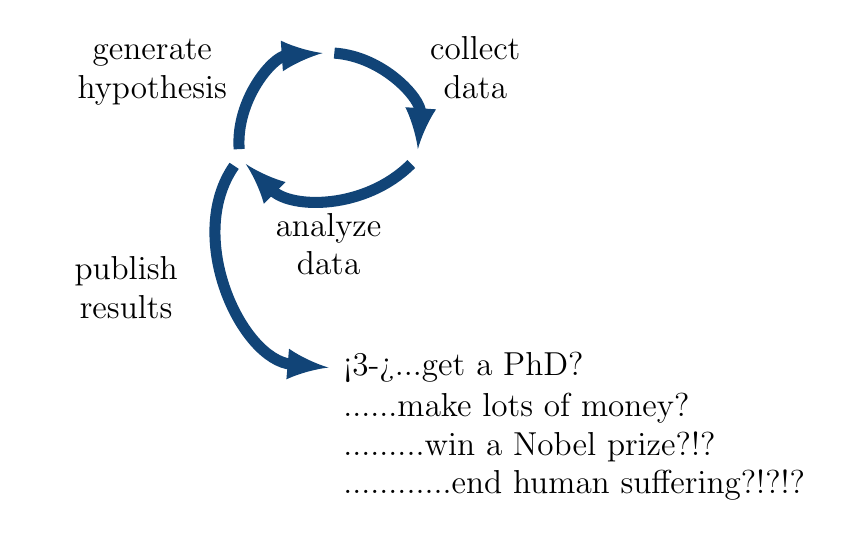
\begin{tikzpicture}[align=center, text depth=.25em, line width=4pt, >=latex, font=\large, color=blue, text=black]
        \node [minimum size=0.2pt, inner sep=0pt] (bottomleft) {};
        \node [minimum size=0.2pt, inner sep=0pt] (top) at ($ (bottomleft) + (50:1.75) $) {};
        \node [minimum size=0.2pt, inner sep=0pt] (bottomright) at ($ (top) + (-50:1.75) $) {};
        \draw [->] (bottomleft) to [bend left=45]
            node[pos=0.2, anchor=south east] {generate \\ hypothesis} (top) ;
        \draw [->] (top) to [bend left=45]
            node[pos=0.8, anchor=south west] {collect \\ data} (bottomright);
        \draw [->] (bottomright) to [bend left=45]
            coordinate[pos=0.3] (midpoint)
            node[midway, anchor=north] {analyze \\ data} (bottomleft);
        \uncover<2->{\draw [->] (bottomleft) to [bend right=60]
            node[midway, anchor=east, minimum width=2.5cm] {publish \\ results} ($ (top) + (-90:4) $)
            node[anchor=west, align=left] (results1) {{\uncover<3->{...get a PhD?}}};}
        \uncover<3->{\node [anchor=north west, align=left] at ($ (results1.west) + (-90:0.4em)$) {......make lots of money? \\
                                                                             .........win a Nobel prize?!? \\
                                                                             ............end human suffering?!?!?};}
    \end{tikzpicture}
\end{frame}

\begin{frame}[t, plain]
    \centerline{
    \begin{tikzpicture}
        \node (rulegraph) {\includegraphics[width=\paperwidth]{figures/rulegraph.pdf}};
        \uncover<2->{\fill [draw=none, fill=white, fill opacity=0.8] (rulegraph.north west) -- (rulegraph.north east) -- (rulegraph.south east) -- (rulegraph.south west) -- (rulegraph.north west) -- cycle;}
        \uncover<2->{\node[] (rule) at (rulegraph.center) {\lstinputlisting[language=Python, backgroundcolor = \color{light-gray}, frame=l, framesep=0.4\textwidth, framerule=0pt, framexbottommargin=1cm]{figures/rule.smk}};}
    \end{tikzpicture}
    }
\end{frame}

\begin{frame}[plain]
    \centerline{\includegraphics[height=\paperheight]{figures/montage.png}}
\end{frame}

\begin{frame}[t,plain]
    \centerline{\includegraphics[width=\paperwidth, trim=0 0 0 0, clip]{figures/zenodo_screenshot.png}}
\end{frame}

\pgfdeclarelayer{backwrapping}
\pgfdeclarelayer{frontwrapping}
\pgfsetlayers{backwrapping,main,frontwrapping}

\tikzset{
        wrapping/.style={
            draw=darkturquoise,
            line cap=round,
            line join=round,
            line width=3pt},
        rnastyle/.style={
            draw=chartreuse!90!black,
            line cap=round,
            line join=round,
            line width=3pt,
            decorate,
            decoration={coil, aspect=0, segment length=15pt}},
        nucleosome/.style={
            fill=sandybrown!60,
            fill opacity=.9,
            draw=none},
        top cylinder/.style={
            fill=sandybrown!85,
            fill opacity=.9
        },
        pics/chromatin/.style 2 args={
            code={
            \foreach \q [remember=\q as \p] in {#1}{
                \begin{scope}[shift={(\q*4.5,0)}, rotate=30]
                    \path [nucleosome]
                        (0.2,1)
                        arc (90:270:0.375 and 1) -- (1,-1)
                        arc (270:90:0.375 and 1) -- cycle;
                    \path [top cylinder]
                        (1.375, 0) arc (0:360:0.375 and 1) -- cycle;

                    \begin{scope}[shift={(0.25,0)}]
                        \begin{pgfonlayer}{backwrapping}
                        \draw [wrapping]
                            (0.5, -1.125)
                            \foreach \i in {360,355,...,180}{ -- (\i/720+0.375*sin -\i, -1.125*cos \i)}
                            [shift={(-0.5,0)}]
                            (0.5, -1.125)
                            \foreach \i in {360,355,...,200}{ -- (\i/720+0.375*sin -\i, -1.125*cos \i)} coordinate (wrapping-start-\q);
                        \end{pgfonlayer}

                        \begin{pgfonlayer}{frontwrapping}
                        \draw [wrapping]
                            (0, -1.125)
                            \foreach \i in {0,5,...,180}{ -- (\i/720+0.375*sin -\i,-1.125*cos \i)}
                            [shift={(0.5,0)}]
                            (0, -1.125)
                            \foreach \i in {0,5,...,200}{ -- (\i/720+0.375*sin -\i,-1.125*cos \i)} coordinate (wrapping-end-\q);
                        \end{pgfonlayer}
                    \end{scope}

                    \ifnum\q=1
                        \draw [wrapping] (wrapping-start-\q) to [bend left=15] ++(-1cm,1cm) ;
                    \fi
                    \ifnum\q>1
                        \draw [wrapping] (wrapping-end-\p) to [bend right=15] coordinate[pos=0.65] (midpoint-\q) (wrapping-start-\q);
                    \fi
                    \ifnum\q=#2
                        \draw [wrapping] (wrapping-end-\q) to [bend right=15] ++(1cm,-1cm);
                    \fi
                \end{scope}
            } % end foreach
            } % end code
        }, % end chromatin
        pol/.pic={
            \shade [%fill=gainsboro,
                top color=gainsboro!85!black,
                bottom color=gainsboro!40!black,
                middle color=gainsboro!85!black,
                   % draw=black,
            opacity=0.98]
                   plot [smooth cycle,
                          tension=0.5] coordinates{(1.5, 0.17)
                                                    (1.6, 1.0)
                                                    (1.3, 1.3)
                                                    (1.7, 2.0)
                                                    (1.4, 2.3)
                                                    %ctd start
                                                    (0, 1.3)
                                                    (-0.5, 2.1)
                                                    (-0.8, 1.8)
                                                    (-1.1, 2.7)
                                                    (-2.5, 2.4)
                                                    (-2.45, 2.2)
                                                    (-1.3, 2.5)
                                                    (-0.9, 1.3)
                                                    (-0.55, 1.8)
                                                    (-0.4, 1.25)
                                                    %ctd end
                                                    (-0.45, 1.1)
                                                    (-1, 0.8)
                                                    (-1.6, 0)
                                                    (-1.25, -0.15)
                                                    (-1.3, -0.55)
                                                    (-0, -0.85)
                                                    (0.5, -0.55)
                                                    (1.6, -0.83)
                                                } -- cycle;
            \coordinate (dnaexit) at (0.3,0.5);
            \node [circle, fill=black!60, minimum width=9pt, inner sep=0pt, outer sep=0pt] at ($(dnaexit) + (-80:0.05)$) {};
        },
        pics/rna/.style={
            code={
                \node [circle, fill=black!60, minimum width=9pt, inner sep=0pt] at (-0.05,0.81) {};
                \draw [rnastyle] (0,0.85) to [bend left=15] ($(0,0.85) + (135:#1)$);
            }
        },
        pics/spt6/.style={
            code={
            \fill [color=#1, opacity=1]
            % \shade [top color=crimson,
            %     bottom color=crimson!60!black,
            %     middle color=crimson,
            %     opacity=0.95]
            plot [smooth cycle, tension=0.5]
            coordinates {(1.5,2.3)
                         (1.7,1.8)
                         (1.5,0.9)
                         (2.6,1.2)
                         (2.4,2.4)
                         (1.5,3.2)
                         % (0.7, 2.6)
                         % (0.7, 2.3)
                         % (-0.6, 1.6)
                         (-1.0,1.7)
                         (-1.8,1.5)
                         (-1.1,0.8)
                         } -- cycle;
            }
        },
        pics/spt5/.style={
            code={
            \fill [color=#1, opacity=1]
            % \shade [top color=darkorange,
            %     bottom color=darkorange!60!black,
            %     middle color=darkorange,
            %     opacity=0.95]
            plot [smooth cycle, tension=0.25]
            coordinates {(1.4,0)
                         (1.5,1.5)
                         (0.9,2)
                         (-1,0.8)
                         (-0.8,0.75)
                         (0,0.95)
                         (0.7,0.25)
                         (0.8,0.1)
                         } -- cycle;
            }
        },
        paf/.pic={
            \fill [color=viridis1, opacity=1]
            % \shade [top color=yellow,
            %     bottom color=yellow!60!black,
            %     middle color=yellow,
            %     opacity=0.95]
            plot [smooth cycle, tension=0.5]
            coordinates {(-0,-0.2)
                         (0.6,0.3)
                         (0.4,0.35)
                         (-0.5,-0.2)
                         (-1.3,-0.2)
                         (-1.3,-1.0)
                         (-0.3,-1.0)
                         (1.0,-1.5)
                         (1.4,-1.0)
                         } -- cycle;
        },
}

\begin{frame}[t]{Transcription}
    \begin{adjustbox}{center}
        \begin{tikzpicture}[scale=0.5, every node/.style={scale=0.5}]
            \pic {chromatin={1, 3, 4, ..., 8}{8}};
            \uncover<2->{
                \pic[rotate=10] at (midpoint-3) {pol};
                \node[font=\Huge] at (midpoint-3 |- 0,5) {initiation};
            }
            \uncover<5->{
                \fill [color=viridis1, rotate=5] ($ (midpoint-3) + (-45:1.5)$) ellipse [x radius=2, y radius=0.8];
                \fill [color=viridis1!70!white, rotate=20] ($ (midpoint-3) + (200:1.4)$) ellipse [x radius=0.5, y radius=0.8];
                \fill [color=viridis1, rotate=15] ($ (midpoint-3) + (150:1.2)$) ellipse [x radius=1, y radius=0.6];
                \fill [color=viridis1!80!white, rotate=-30] ($ (midpoint-3) + (80:2.0)$) ellipse [x radius=1, y radius=0.6];
            }
            \uncover<2->{
                \draw [wrapping, rotate=10] (midpoint-3) to [bend left=9] (wrapping-end-1);
                \draw [wrapping, rotate=10] (dnaexit) to [bend left=60] (midpoint-3);
            }
            \uncover<3->{
                \pic at (midpoint-5) {pol};
                \node [font=\Huge] at (midpoint-5 |- 0,5) {elongation};
            }
            \uncover<5>{
                \pic at (midpoint-5) {paf};
                \pic at (midpoint-5) {spt5={viridis1!70!white}};
                \pic at (midpoint-5) {spt6={viridis1!93!white}};
            }
            \uncover<3->{
                \draw [wrapping] (midpoint-5) to [bend left=10] (wrapping-end-4);
                \draw [wrapping] (dnaexit) to [bend left=60] (midpoint-5);
                \pic at (midpoint-5) {rna={6}};
            }
            \uncover<4->{
                \pic at (midpoint-7) {pol};
                \node [font=\Huge] at (midpoint-7 |- 0,5 ) {termination};
            }
            \uncover<5->{
                \fill [color=viridis1!90!white, rotate=30] ($ (midpoint-7) + (-80:0.9)$) ellipse [x radius=0.9, y radius=0.6];
                \fill [color=viridis1, rotate=-10] ($ (midpoint-7) + (200:1)$) ellipse [x radius=0.4, y radius=0.6];
                \fill [color=viridis1!50!white, rotate=30] ($ (midpoint-7) + (35:1.7)$) ellipse [x radius=0.7, y radius=1];
            }
            \uncover<4->{
                \draw [wrapping] (midpoint-7) to [bend left=10] (wrapping-end-6);
                \draw [wrapping] (dnaexit) to [bend left=60] (midpoint-7);
                \pic at (midpoint-7) {rna={10}};
            }
            \draw [line width=2pt, color=gray!90] (midpoint-3 |- 0,-3) -- coordinate[pos=0.07] (orfstart) coordinate[pos=0.85] (notch) coordinate[pos=0.93] (orfend) (midpoint-7 |- 0,-3);
            \fill [fill=gray!45] ($(orfstart) + (-90:0.6)$) --
                                 ($(orfstart) + (90:0.6)$) --
                                 ($(notch) + (90:0.6)$) --
                                 (orfend) --
                                 ($(notch) + (-90:0.6)$) --
                                 cycle;
            \node [font=\Huge] at ($ (orfstart)!0.5!(orfend) $) {a gene};
        \end{tikzpicture}
    \end{adjustbox}
\end{frame}

\begin{frame}[t,plain]
    \begin{adjustbox}{center}
        \begin{tikzpicture}
            \node [anchor=south] (figure) {\includegraphics[width=\paperwidth]{../../structures/elongating_transcription_complex_with_nucleosome.png}};
            \node [align=left,
                   font=\footnotesize] (figure){Vos \textit{et al.} (2018). \textit{Nature} \\
                                                   Farnung \textit{et al.} (2018). \textit{Nat. Commun.}};
        \end{tikzpicture}
    \end{adjustbox}
\end{frame}

\begin{frame}{Spt6 project collaborators}
    \begin{description}[align=right, leftmargin=!, labelwidth=0.5\textwidth]
        \item [Steve Doris] TSS-seq and ChIP-nexus
        \item [Olga Viktorovskaya] MNase-seq
        \item [Magdalena Murawska] NET-seq
        \item [Dan Spatt] Northern, Western, and ChIP experiments
    \end{description}
\end{frame}

\begin{frame}{The \textbf{\textit{spt6-1004}} mutant expresses \textbf{intragenic transcripts}}
    \centering
    \begin{columns}
        \begin{column}{0.5\textwidth}
            \includegraphics<1->[width=\textwidth]{figures/presentation/presentation_six_spt6_western.pdf}
        \end{column}
        \begin{column}{0.5\textwidth}
            \centering
            \uncover<2->{
            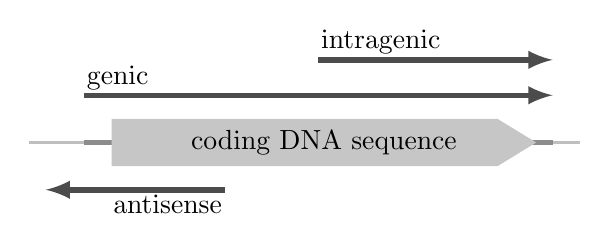
\begin{tikzpicture}[x=7cm, y=0.3cm, >=latex, font=\normalsize, text=black]
                \draw [line width=1pt, color=gray!50] (0,0) -- (1,0);
                \draw [line width=2pt, color=gray!90] (0.1,0) coordinate (genicstart) -- (0.95,0) coordinate (genicend);
                \fill [fill=gray!45] (0.15, -1) -- coordinate[midway] (orfstart) (0.15, 1) -- (0.85, 1) -- (0.92, 0) coordinate(orfend) -- (0.85, -1) -- cycle;
                \node at ($ (orfstart)!0.5!(orfend) $) {coding DNA sequence};
                \draw [line width=2pt, ->, color=black!70, text=black] ($ (genicstart) + (90:2)$)
                    node[above, anchor=south west, inner xsep=0, inner ysep=1pt] {genic} -- ($ (genicend) + (90:2)$ );
                \uncover<3->{
                \draw [line width=2pt, ->, color=black!70, text=black] ($ (genicstart)!0.5!(genicend) + (90:3.5)$)
                    node[above, anchor=south west, inner xsep=0, inner ysep=1pt] {intragenic} -- ($ (genicend) + (90:3.5)$ );
                \draw [line width=2pt, ->, color=black!70, text=black] ($ (genicstart)!0.3!(genicend) + (-90:2)$)
                    node[below, anchor=north east, inner xsep=0, inner ysep=1pt] {antisense} -- ($ (0,0)!0.3!(genicstart) + (-90:2)$ );
                % \draw [line width=1pt, ->] ($ (0,0)!0.8!(genicstart) + (-90:1)$)
                %     node[below, anchor=north east, inner xsep=0, inner ysep=1pt] {intergenic} -- ($ (0,0) + (-90:1)$ );
                }
            \end{tikzpicture}
        }
        \end{column}
    \end{columns}
\end{frame}

\begin{frame}[t]
    \begin{tikzpicture}
        \node<1-2>[inner sep=0] (marker) {\includegraphics[width=\textwidth]{figures/presentation/presentation_six_aat_assay_comparison.pdf}};
        \fill<1>[white] (marker.south east) rectangle (-6.55cm, -0.2cm);
    \end{tikzpicture}
\end{frame}

\begin{frame}[t]
    \begin{tikzpicture}
        \node<1-2>[inner sep=0] (marker) {\includegraphics[width=\textwidth]{figures/presentation/presentation_six_tss_seq_heatmaps.pdf}};
        \fill<1>[white] (marker.south east) rectangle (marker.north);
    \end{tikzpicture}
\end{frame}

\begin{frame}{Downregulation of genic TSSs in \textit{spt6-1004}:}
    \centering
    \begin{columns}
        \begin{column}{0.5\textwidth}
            \includegraphics<1->[width=\textwidth]{figures/presentation/presentation_six_tss_diffexp_summary.pdf}
        \end{column}
        \begin{column}{0.5\textwidth}
            \includegraphics<2>[width=\textwidth]{figures/presentation/presentation_six_tss_expression_levels.pdf}
        \end{column}
    \end{columns}
\end{frame}

\begin{frame}{Measuring transcription initiation with TFIIB ChIP-nexus}
    \begin{tikzpicture}
        \node[inner sep=0] at (0,0) {\includegraphics[width=15cm]{figures/presentation/presentation_six_tfiib_spreading_swc0001.pdf}};
        \fill[white] (0.3,-0.1) rectangle (3.5, 0.50);
    \end{tikzpicture}
\end{frame}

\begin{frame}[t]
    \centering
    \includegraphics[width=10.5cm]{figures/presentation/presentation_six_tfiib_heatmap.pdf}
\end{frame}

\begin{frame}{TFIIB binding changes dramatically in \textit{spt6-1004}:}
    \begin{tikzpicture}
        % \node<1>[inner sep=0] at (0,0) {\includegraphics[width=15cm]{figures/presentation/presentation_six_tfiib_spreading_swc0001.pdf}};
        % \fill<1>[white] (0.3,-0.1) rectangle (3.5, 0.50);
        \node[inner sep=0] at (0,0) {\includegraphics[width=15cm]{figures/presentation/presentation_six_tfiib_spreading_swc0002.pdf}};
    \end{tikzpicture}
\end{frame}

\begin{frame}{new intragenic initiation explains most intragenic transcripts}
    \includegraphics[width=\textwidth]{figures/presentation/presentation_six_tss_v_tfiib.pdf}
\end{frame}

\begin{frame}
    \begin{tikzpicture}
        \node<1>[inner sep=0] at (0,0) {\includegraphics[width=\textwidth]{figures/presentation/presentation_six_mnase_metagene0001.pdf}};
        \fill<1>[white] (-0.7,0.49) rectangle (2.2, 1.01);
        \node<2>[inner sep=0] at (0,0) {\includegraphics[width=\textwidth]{figures/presentation/presentation_six_mnase_metagene0002.pdf}};
    \end{tikzpicture}
\end{frame}

\begin{frame}
    \centering
    \begin{tikzpicture}
        \node<1-3>[inner sep=0] (marker) at (0,0) {\includegraphics[width=\textwidth]{figures/presentation/presentation_six_intragenic_mnase_metagenes.pdf}};
        \fill<1-3>[white] (2.8,1.15) rectangle (marker.north east);
        \fill<1>[white] (-1.8,-3.825) rectangle (marker.north east);
        \fill<1-2>[white] (2.8,-3.825) rectangle (marker.north east);
    \end{tikzpicture}
\end{frame}

\begin{frame}{Features of intragenic promoters}
    \centering
    \includegraphics[width=\textwidth]{figures/presentation/presentation_six_intragenic_gc.pdf}
\end{frame}

\begin{frame}{Features of intragenic promoters}
    \centering
    \begin{tikzpicture}
        \node<1>[inner sep=0] at (0,0) {\includegraphics[width=12cm]{figures/presentation/presentation_six_intragenic_tata0001.pdf}};
        \fill<1>[white] (-3.5,-0.40) rectangle (-1.1, 0.45);
        \fill<1>[white] (-3.5,0.44) rectangle (-3, 0.495);
        \node<2>[inner sep=0] at (0,0) {\includegraphics[width=12cm]{figures/presentation/presentation_six_intragenic_tata0002.pdf}};
    \end{tikzpicture}
\end{frame}

\begin{frame}{Features of intragenic promoters}
    \centering
    \includegraphics[width=12cm]{figures/presentation/presentation_six_tss_seqlogos.pdf}
\end{frame}

\begin{frame}{Spt6 summary and model}
\end{frame}

\begin{frame}[t,plain]
    \begin{adjustbox}{center}
        \begin{tikzpicture}
            \node [anchor=south] (figure) {\includegraphics[width=\paperwidth]{../../structures/elongating_transcription_complex_with_nucleosome.png}};
            \node [align=left,
                   font=\footnotesize] (figure){Vos \textit{et al.} (2018). \textit{Nature} \\
                                                   Farnung \textit{et al.} (2018). \textit{Nat. Commun.}};
        \end{tikzpicture}
    \end{adjustbox}
\end{frame}

\begin{frame}{Spt5 project collaborators}
    \begin{description}[align=right, leftmargin=!, labelwidth=0.5\textwidth]
        \item [Ameet Shetty] NET-seq,\\ChIP-seq,\\RNA-seq,\\TSS-seq,\\MNase-seq,\\etc.
    \end{description}
\end{frame}

\begin{frame}{Spt5 depletion system}
    \centering
    \begin{columns}
        \begin{column}{0.45\textwidth}
            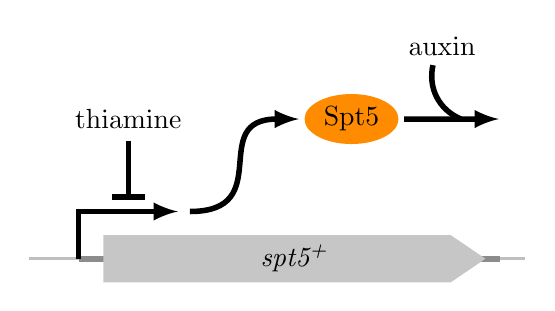
\begin{tikzpicture}[x=6.3cm, y=0.3cm, >=latex, font=\normalsize, text=black]
                \draw [line width=1pt, color=gray!50] (0,0) -- (1,0);
                \draw [line width=2pt, color=gray!90] (0.1,0) coordinate (genicstart) -- (0.95,0) coordinate (genicend);
                \fill [fill=gray!45] (0.15, -1) -- coordinate[midway] (orfstart) (0.15, 1) -- (0.85, 1) -- (0.92, 0) coordinate(orfend) -- (0.85, -1) -- cycle;
                \node at ($ (orfstart)!0.5!(orfend) $) {\textit{spt5\textsuperscript{+}}};
                \draw [->, line width=2pt] (genicstart) -- ($ (genicstart) + (90:2)$) --
                    node[midway] (promoter) {} ++(0.2,0) node (exprstart) {};
                \draw [|-, line width=2pt] (promoter) -- ++(0, 3) node [anchor=south] (thiamine) {thiamine};
                \draw (0.95,0 |- thiamine) node [outer sep=0pt, inner sep=0pt] (degraded) {\scalebox{2}{$\varnothing$}};
                \node [ellipse, fill=darkorange, inner sep=2pt, outer sep=2pt] (spt5) at ($ (thiamine)!0.6!(degraded) $) {Spt5};
                \draw [->, line width=2pt] (exprstart) .. controls ++(0.2,0) and ($ (thiamine)!0.35!(spt5) $) .. (spt5);
                \draw [->, line width=2pt] (spt5) --
                    coordinate[pos=0.4] (auxincoord)
                    coordinate[pos=0.6] (auxintarget) (degraded);
                \draw (auxincoord |- 0,9) node (auxin) {auxin};
                \draw [line width=2pt] (auxin) to [bend right=40] (auxintarget);
            \end{tikzpicture}
        \end{column}
        \begin{column}{0.55\textwidth}
            \pause
            \includegraphics[width=\textwidth]{figures/presentation/presentation_five_spt5_depletion.pdf}
        \end{column}
    \end{columns}
\end{frame}

\begin{frame}{Elongation defects upon Spt5 depletion}
    \centering
    \includegraphics[width=12cm]{figures/presentation/presentation_five_netseq_meta.pdf}
\end{frame}

\begin{frame}{Trapped Pol II is enriched for CTD serine 5 phosphorylation}
    \includegraphics[width=\textwidth]{figures/presentation/presentation_five_rnapii_phosphomark_enrichment.pdf}
\end{frame}

\begin{frame}{Evidence for premature termination upon Spt5 depletion}
    \centering
    \includegraphics[width=12cm]{figures/presentation/presentation_five_rnaseq_metagene.pdf}
\end{frame}

\begin{frame}[t]
    \centering
    \includegraphics[width=10.5cm]{figures/presentation/presentation_five_rnaseq_heatmaps.pdf}
\end{frame}

\begin{frame}[t]
    \includegraphics[width=\textwidth]{figures/presentation/presentation_five_antisense_heatmaps.pdf}
\end{frame}

\begin{frame}[t]
    \includegraphics[width=\textwidth]{figures/presentation/presentation_five_mnase_metagene.pdf}
\end{frame}

\begin{frame}{Spt5 summary and model}
\end{frame}

\begin{frame}{WT intragenic transcription}
\end{frame}

\begin{frame}{project collaborators}
    \begin{description}[align=right, labelwidth=0.5\textwidth, leftmargin=!]
        \item [Steve Doris] TSS-seq and ChIP-nexus
        \item [Dan Spatt] polyribosome fractionation,\\competitive growth assays,\\and Northern blots
        \item [James Warner] Northern blots
    \end{description}
\end{frame}

\begin{frame}[t]
    \includegraphics[width=\textwidth]{figures/presentation/presentation_stress_tfiib_ridgelines.pdf}
\end{frame}

\begin{frame}
    \includegraphics[width=\textwidth]{figures/presentation/presentation_stress_tfiib_coverage.pdf}
\end{frame}

\begin{frame}[t]
    \includegraphics[width=\textwidth]{figures/presentation/presentation_stress_promoter_tss_expression.pdf}
\end{frame}

\begin{frame}[t]
    \includegraphics[width=\textwidth]{figures/presentation/presentation_stress_promoter_tss_polyenrichment.pdf}
\end{frame}

\begin{frame}[t,plain]
    \begin{adjustbox}{center}
        \begin{tikzpicture}
            \node [anchor=south east] (figure) {\includegraphics[width=\textwidth]{figures/presentation/presentation_stress_dsk2_summary.pdf}};
            \node [anchor=north east, font=\footnotesize] (figure){MNase-ChIP-seq: Weiner \textit{et al.} (2015). \textit{Mol. Cell}};
        \end{tikzpicture}
    \end{adjustbox}
\end{frame}

\begin{frame}
    \begin{columns}
        \begin{column}{0.5\textwidth}
            \includegraphics[width=\textwidth]{figures/presentation/presentation_stress_dsk2_pace_northern.pdf}
        \end{column}
        \begin{column}{0.5\textwidth}
        \end{column}
    \end{columns}
\end{frame}

\begin{frame}
    \includegraphics[width=\textwidth]{figures/presentation/presentation_stress_diamide_fitnesscomp.pdf}
\end{frame}

\begin{frame}{Summary}
\end{frame}

\begin{frame}{Acknowledgements}
\end{frame}

\end{document}
